\documentclass{standalone}

\usepackage{siunitx}
\usepackage{tikz} % To generate the plot from csv
\usepackage{varwidth}
\usetikzlibrary{shapes,arrows}
\usetikzlibrary{backgrounds}
\usetikzlibrary{matrix, positioning, fit}
\usetikzlibrary{patterns}
\definecolor{forestgreen}{rgb}{0.0, 0.5, 0.0}

\tikzstyle{smallcircle} =[fill=black!100, text=white, circle, inner sep=1pt, minimum size=0.1em]
\tikzstyle{ourcircle} = [draw, semicircle, inner sep=0pt,minimum size=2pt]
\tikzstyle{dullblock} = [draw, fill=black!20, circle, minimum height=2em, minimum width=2em]
\tikzstyle{block} = [draw=black, rounded corners, thick, line width=0.3mm, rectangle, minimum height=10em, minimum width=7em]
\tikzstyle{blocksmall} = [draw=black, thick, line width=0.5mm, rectangle, minimum height=6em, minimum width=3em, fill=white]
\tikzstyle{group} = [draw=black, line width=0.3mm, rectangle, minimum height=2em, minimum width=2em]
\tikzstyle{textblock} = [draw, fill=black!20, rectangle, rounded corners]
\tikzstyle{rectblock} = [draw, rectangle, minimum height=1.3em]
\tikzstyle{plain} = []
\tikzstyle{decisionblock} = [draw, diamond, fill=black!20]
\tikzstyle{input} = [draw, thick, fill=blue!20, circle, minimum size=1pt]
\tikzstyle{output} = [draw, fill=blue!20, circle, minimum size=1pt]
\tikzstyle{pinstyle} = [pin edge={to-,thin,black}]
\tikzset{toprule/.style={%
        execute at end cell={%
            \draw [line cap=rect,#1] (\tikzmatrixname-\the\pgfmatrixcurrentrow-\the\pgfmatrixcurrentcolumn.north west) -- (\tikzmatrixname-\the\pgfmatrixcurrentrow-\the\pgfmatrixcurrentcolumn.north east);%
        }
    },
    bottomrule/.style={%
        execute at end cell={%
            \draw [line cap=rect,#1] (\tikzmatrixname-\the\pgfmatrixcurrentrow-\the\pgfmatrixcurrentcolumn.south west) -- (\tikzmatrixname-\the\pgfmatrixcurrentrow-\the\pgfmatrixcurrentcolumn.south east);%
        }
    }
}


\begin{document}

    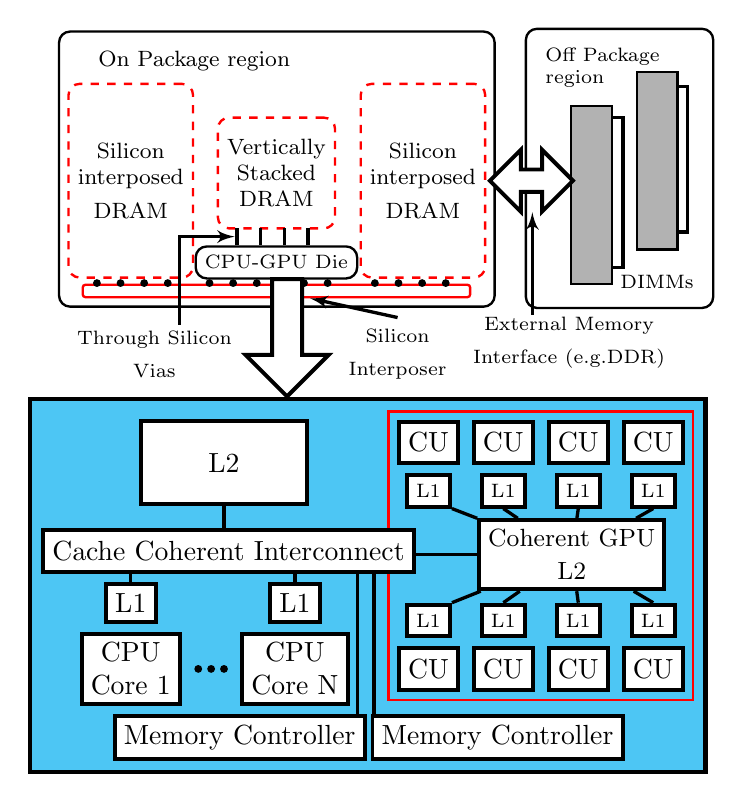
\begin{tikzpicture}[auto, >=latex']
        %CPU
        \node [blocksmall, minimum height=1em, minimum width=1em] (cpu1) {\begin{varwidth}{4cm}\centering{CPU\\ Core 1} \end{varwidth}};
        \node [blocksmall, above = 0.1cm of cpu1, minimum height=1em, minimum width=1em] (l11){\begin{varwidth}{4cm} \centering{L1} \end{varwidth}};
        
        %\node [blocksmall, right = 0.1cm of cpu1, minimum height=1em, minimum width=1em] (cpu2) {\begin{varwidth}{4cm} \centering{CPU\\ Core 2} \end{varwidth}};
        %\node [blocksmall, above = 0.1cm of cpu2, minimum height=1em, minimum width=1em] (l12){\begin{varwidth}{4cm} \centering{L1} \end{varwidth}};
        
        \node [smallcircle, right=0.15cm of cpu1] (dot1) {};
        \node [smallcircle, right=0.05cm of dot1] (dot2) {};
        \node [smallcircle, right=0.05cm of dot2] (dot3) {};
        
        %\node [blocksmall, right = 0.1cm of cpu2, minimum height=1em] (cpu3){\begin{varwidth}{4cm} \centering{CPU\\ Core 3} \end{varwidth}};
        %\node [blocksmall, above = 0.1cm of cpu3, minimum height=1em] (l13){\begin{varwidth}{4cm} \centering{L1} \end{varwidth}};
        
        \node [blocksmall, right = 0.15cm of dot3, minimum height=1em, minimum width=1em] (cpu4){\begin{varwidth}{4cm} \centering{CPU\\ Core N} \end{varwidth}};
        \node [blocksmall, above = 0.1cm of cpu4, minimum height=1em, minimum width=1em] (l14){\begin{varwidth}{4cm} \centering{L1} \end{varwidth}};
        \node [blocksmall, above = 2.01cm of dot3, minimum height=3em, minimum width=6em] (l24){\begin{varwidth}{4cm} \centering{L2} \end{varwidth}};
        
       % \begin{scope}[on background layer]
            %\node[group, inner sep = 3pt, line width=0.3mm, draw=red, yshift=1em, fit=(cpu1)(cpu2)(cpu3)(cpu4)(l11)(l12)(l13)(l14)(l24)] (grpcpu) {};
       % \end{scope}
        
        
        %GPU
        \node [blocksmall, right = 0.6cm of cpu4, minimum height=1.5em, minimum width=1em] (sm1) {CU};
        \node [blocksmall, above = 0.1cm of sm1, minimum height=1pt, minimum width=1em] (sm1l1) {\scriptsize{L1}};
        \node [blocksmall, right = 0.15cm of sm1, minimum height=1.5em, minimum width=1em] (sm2) {CU};
        \node [blocksmall, above = 0.1cm of sm2, minimum height=1em, minimum width=1em] (sm2l1) {\scriptsize{L1}};
        \node [blocksmall, right = 0.15cm of sm2, minimum height=1.5em, minimum width=1em] (sm3) {CU};
        \node [blocksmall, above = 0.1cm of sm3, minimum height=1em, minimum width=1em] (sm3l1) {\scriptsize{L1}};
        \node [blocksmall, right = 0.15cm of sm3, minimum height=1.5em, minimum width=1em] (sm4) {CU};
        \node [blocksmall, above = 0.1cm of sm4, minimum height=1em, minimum width=1em] (sm4l1) {\scriptsize{L1}};
        \node [blocksmall, above = 2.3cm of sm1, minimum height=1.5em, minimum width=1em] (sm5) {CU};
        \node [blocksmall, below = 0.1cm of sm5, minimum height=1em, minimum width=1em] (sm5l1) {\scriptsize{L1}};
        \node [blocksmall, right = 0.15cm of sm5, minimum height=1.5em, minimum width=1em] (sm6) {CU};
        \node [blocksmall, below = 0.1cm of sm6, minimum height=1em, minimum width=1em] (sm6l1) {\scriptsize{L1}};
        \node [blocksmall, right = 0.15cm of sm6, minimum height=1.5em, minimum width=1em] (sm7) {CU};
        \node [blocksmall, below = 0.1cm of sm7, minimum height=1em, minimum width=1em] (sm7l1) {\scriptsize{L1}};
        \node [blocksmall, right = 0.15cm of sm7, minimum height=1.5em, minimum width=1em] (sm8) {CU};
        \node [blocksmall, below = 0.1cm of sm8, minimum height=1em, minimum width=1em] (sm8l1) {\scriptsize{L1}};  
        
        \node [blocksmall, minimum height=1.1em, minimum width=6em] at (5.6,1.45)
        (l2gpu) {\begin{varwidth}{4cm} \centering{\small{Coherent GPU \\L2}}\end{varwidth}};
        
         %\begin{scope}[on background layer]
            \node[group, inner sep = 3pt, line width=0.3mm, draw=red, fit=(sm1)(sm1l1)(sm2)(sm2l1)(sm3)(sm3l1)(sm4)(sm4l1)(sm5)(sm5l1)(sm6)(sm6l1)(sm7)(sm7l1)(sm8)(sm8l1)(l2gpu)] (grpgpu) {};
         %\end{scope}                        
        
        
        %Interconnect
        \node [blocksmall, minimum height=1.5em, minimum width=10.7em] at (1.24,1.5)
        (interconnect) {Cache Coherent Interconnect};
                
        %Connections to interconnect
        \draw [-,very thick] (l11.north) to ++(0, 0.15); 
        \draw [-, very thick] (l24.south) to ++(0, -0.3);
        \draw [-, very thick] (l2gpu.west) to ++(-0.82,0);
        \draw [-, very thick] (l14.north) to ++(0, 0.15);
        %\draw [-, very thick] (l13.north) to ++(0, 0.15);
        %\draw [-, very thick] (l12.north) to ++(0, 0.15);
        
        % Memory Controller
        \node [blocksmall, minimum height=1em, minimum width=9em, below=0.1cm of cpu4, xshift=-2em] (mc1){\begin{varwidth}{4cm} \centering{Memory Controller} \end{varwidth}};
        \node [blocksmall, minimum height=1em, minimum width=9em, right=0.05cm of mc1] (mc2){\begin{varwidth}{4cm} \centering{Memory Controller} \end{varwidth}};  
        
        %\draw [-, very thick] (-0.78,-0.6) to (-0.78, 1.5) to (interconnect.west);
        \draw [-, very thick] (2.88,-0.6) to (2.88, 1.25);
        \draw [-, very thick] (3.09,-0.6) to (3.09, 1.25);
        
        %Chip
        \begin{scope}[on background layer]
             \node[group, inner sep = 4pt, line width=0.6mm, fill=cyan!70, fit=(cpu1)(cpu4)(l11)(l14)(l24)(interconnect)(mc1)(mc2)(grpgpu)] (grpchip) {};
        \end{scope}
        
        %DRAM Cache  
        \node [block, draw=red, dashed, minimum height=7em, minimum width=4em] at (0,6.2) (sid){\begin{varwidth}{4cm} \centering{\footnotesize{Silicon\\ interposed\\ DRAM}} \end{varwidth}};
        
        \node [block, draw=red, right = 2.1cm of sid, dashed, minimum height=7em, minimum width=4em] (sid1){\begin{varwidth}{4cm} \centering{\footnotesize{Silicon\\ interposed\\ DRAM}} \end{varwidth}};
        
        \node [block, draw=red, minimum height=0.1pt, rounded corners=1pt, inner sep=1pt, minimum width=14em] at (1.85, 4.8) (blk1){\begin{varwidth}{4cm} \end{varwidth}};
        
        \node [block, draw=black, above = 0.05cm of blk1, minimum height=0.1em, minimum width=1em] (cpud){\begin{varwidth}{4cm} \centering{\scriptsize{CPU-GPU Die}} \end{varwidth}};
        
        \node [block, draw=red, above = 0.2cm of cpud, minimum height=4em, dashed, minimum width=4em] (vsd) {\begin{varwidth}{4cm} \centering{\footnotesize{Vertically\\ Stacked\\ DRAM\\}} \end{varwidth}};
        
        \node [blocksmall,opacity=0,text opacity=1, draw=white, above = 0.01cm of sid.north east, minimum height=1em, minimum width=0.2em] (lbl3){\footnotesize{On Package region}};
        
        \node[group, inner sep = 3pt, rounded corners, fit=(sid)(vsd)(sid1)(cpud)(blk1)(lbl3)] (g1) {};
        
        % TSV        
        \draw [-,very thick] (1.35,5.38) to (1.35,5.6);
        \draw [-,very thick] (1.65,5.38) to (1.65,5.6);
        \draw [-,very thick] (1.95,5.38) to (1.95,5.6);
        \draw [-,very thick] (2.25,5.38) to (2.25,5.6);
        
        % semicircles
        \node [smallcircle] at (-0.43,4.9) (s4) {};
        \node [smallcircle] at (-0.13,4.9) (s1) {};
        \node [smallcircle] at (0.17,4.9) (s2) {};
        \node [smallcircle] at (0.47,4.9) (s3) {};
        %\node [smallcircle] at (0.7,4.9) (s3) {};
        %\node [smallcircle] at (1.0,4.9) (s4) {};

        \node [smallcircle] at (1,4.9) (s5) {};
        \node [smallcircle] at (1.3,4.9) (s6) {};
        \node [smallcircle] at (1.6,4.9) (s7) {};
        \node [smallcircle] at (1.9,4.9) (s8) {};
        \node [smallcircle] at (2.2,4.9) (s9) {};
        \node [smallcircle] at (2.5,4.9) (s10) {};

        \node [smallcircle] at (3.1,4.9) (s11) {};
        \node [smallcircle] at (3.4,4.9) (s12) {};
        \node [smallcircle] at (3.7,4.9) (s13) {};
        \node [smallcircle] at (4,4.9) (s14) {};
        %\node [smallcircle] at (4.3,4.9) (s15) {};
        
        % GPU L1 to L2 connections
        \draw [-,very thick] (sm1l1.north east) -- (l2gpu);
        \draw [-,very thick] (sm2l1.north) -- (l2gpu);
        \draw [-,very thick] (sm3l1.north) -- (l2gpu);
        \draw [-,very thick] (sm4l1.north) -- (l2gpu);
        \draw [-,very thick] (sm5l1.south east) -- (l2gpu);
        \draw [-,very thick] (sm6l1.south) -- (l2gpu);
        \draw [-,very thick] (sm7l1.south) -- (l2gpu);                
        \draw [-,very thick] (sm8l1.south) -- (l2gpu);
        
        % Off package Region
        \node [blocksmall, draw=black!30, fill=black!30, minimum height=0.5em, minimum width=0.5em] at (5.85,5.15)(mm1){};
        \node [blocksmall, draw=black!30, fill=black!30, above = 0.15cm of mm1, minimum height=0.5em, minimum width=0.5em] (mm2){};
        \node [blocksmall, draw=black!30, fill=black!30, above = 0.15cm of mm2, minimum height=0.5em, minimum width=0.5em] (mm3){};
        \node [blocksmall, draw=black!30, fill=black!30, above = 0.15cm of mm3, minimum height=0.5em, minimum width=0.5em] (mm4){};
        \node [blocksmall, draw=black!30, fill=black!30, above = 0.15cm of mm4, minimum height=0.5em, minimum width=0.5em] (mm5){};
        %\node [blocksmall, draw=black!30, fill=black!30, above = 0.2cm of mm5, minimum height=0.5em, minimum width=0.5em] (mm6){};

        \node [blocksmall, draw=black!30, fill=black!30, minimum height=0.5em, right = 0.55cm of mm2, minimum width=0.5em] (mm7){};
        \node [blocksmall, draw=black!30, fill=black!30, above = 0.15cm of mm7, minimum height=0.5em, minimum width=0.5em] (mm8){};
        \node [blocksmall, draw=black!30, fill=black!30, above = 0.15cm of mm8, minimum height=0.5em, minimum width=0.5em] (mm9){};
        \node [blocksmall, draw=black!30, fill=black!30, above = 0.15cm of mm9, minimum height=0.5em, minimum width=0.5em] (mm10){};
        \node [blocksmall, draw=black!30, fill=black!30, above = 0.15cm of mm10, minimum height=0.5em, minimum width=0.5em] (mm11){};
       % \node [blocksmall, draw=black!30, fill=black!30, above = 0.2cm of mm11, minimum height=0.5em, minimum width=0.5em] (mm12){};
        \begin{scope}[on background layer]
            \node [blocksmall, opacity=0,text opacity=1, draw=white, below = 0.3cm of mm7, minimum height=1em, minimum width=1.2em] (lbl1){\scriptsize{DIMMs}};
        \end{scope}
        \begin{scope}[on background layer]
            \node [blocksmall, opacity=0,text opacity=1, draw=white, above = 0.21cm of mm5.north east, minimum height=0.1em, minimum width=0.1em] (lbl2){\begin{varwidth}{4cm} \scriptsize{Off Package\\region}\end{varwidth}};
       \end{scope}
        
        % Memory Grouping
        \begin{scope}[on background layer]
              \node[group, minimum width=0.1em, minimum height=0.1em, fill=black!30, fit=(mm1)(mm2)(mm3)(mm4)(mm5)] (mmgrp1) {};
        \end{scope}
        \begin{scope}[on background layer]
              \node[group, minimum width=0.1em, minimum height=0.1em, fill=black!30, fit=(mm7)(mm8)(mm9)(mm10)(mm11)] (mmgrp2) {};
        \end{scope}
        \node[group, inner sep = 3pt, rounded corners, line width=0.3mm, fit=(mmgrp1)(mmgrp2)(lbl1)(lbl2)] (mmgrp3) {};
        %\node[group, inner sep = 3pt, line width=0.3mm, fit=(mmgrp1)(mmgrp2)] (mmgrp3) {};
        
        %\draw [-,very thick] (7.9,6.5) to (7.9, 6.3) to (11.3,6.3) to (11.3,6.5);
        %\draw [-,very thick] (8.5,5.35) to (8.5, 5.15) to (11.9,5.15) to (11.9,5.35);
        \draw [-,very thick] (6.1, 5.1) to (6.25, 5.1) to (6.25, 7.0) to (6.1, 7.0);
        \draw [-,very thick] (6.93, 5.55) to (7.07, 5.55) to (7.07, 7.4) to (6.93, 7.4);
        
        % Big Arrows
        \node[single arrow, draw, below = 0.1mm of cpud.south, xshift=1em,
        yshift=-1.8em, rotate=-90, minimum height=4.24em, minimum width=3em, line width=0.5mm, fill=white](arrow1){};
        \node[double arrow, draw, right = 0.1mm of sid1.east,
        yshift=0em, rotate=0, minimum height=3em, minimum width=1.3em, line width=0.5mm, fill=white](arrow2){};
        
        % Labels
        \node [blocksmall, opacity=0,text opacity=1, draw=white, minimum height=1em, minimum width=1.2em] at (0.3,4.0)
        (lbl4){\begin{varwidth}{4cm} \centering{\scriptsize{Through Silicon\\Vias}}\end{varwidth}};
        \node [blocksmall, opacity=0,text opacity=1, draw=white, right=1.2cm of lbl4, minimum height=1em, minimum width=1.2em] (lbl5) {\begin{varwidth}{4cm} \centering{\scriptsize{Silicon\\Interposer}}\end{varwidth}};
        \node [blocksmall, opacity=0,text opacity=1, draw=white, right=0.1cm of lbl5, minimum height=1em, minimum width=1.2em, yshift=0.4em, inner sep=2pt] (lbl6) {\begin{varwidth}{4cm} \centering{\scriptsize{External Memory \\Interface (e.g.DDR)}} \end{varwidth}};
        
        % Label Arrows
        \draw[->, very thick] (lbl5.north) to (blk1);
        \draw[<-, very thick] (5.1, 5.8) to [in=90,out=-90] ++(0,-1.3);
        \draw[<-, very thick] (1.32,5.49) to [in=0,out=180] ++(-0.7,0) to [in=90,out=-90] ++(0,-1.12);
        
    \end{tikzpicture}
\end{document}
